\documentclass[a4paper, 12pt]{exam}

\makeatletter
\expandafter\providecommand\expandafter*\csname ver@framed.sty\endcsname
{2003/07/21 v0.8a Simulated by exam}
\makeatother

\usepackage{xcolor}
\usepackage{minted}
\usepackage[utf8]{inputenc}
\usepackage{tikz}
\usepackage{caption}
\usepackage{gensymb}
\usepackage{lmodern}
\usepackage{multirow}
\usepackage{booktabs}
\usepackage{array}
\usepackage{adjustbox}
\usepackage{upquote}
\usepackage{amsmath}
\usepackage[hidelinks]{hyperref}
\usetikzlibrary{mindmap,shadows, shapes, arrows, automata, positioning, backgrounds}

\renewcommand{\refname}{\selectfont\normalsize References} 
\pagestyle{headandfoot}

\header{\textbf{Problem Sheet: Automata}}{}{Graph Theory}
\footer{}{Page \thepage\ of \numpages}{}
\marksnotpoints
\pointsinrightmargin

\begin{coverpages}
\end{coverpages}

\begin{document}

%\printanswers

\begin{questions}


\question
  Draw a DFA that accepts all strings over $\{a,b\}$ that have at least three $a$'s~\cite{sipser96}.
  
  \begin{solution}
    \begin{center}
      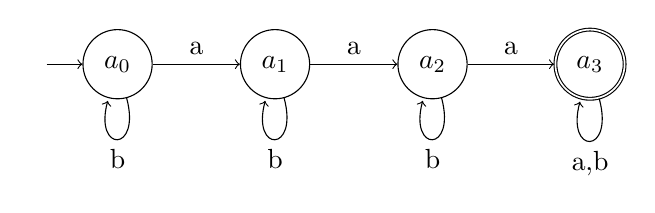
\begin{tikzpicture}[auto, on grid, node distance=2cm, initial text=]
        \node[state, initial]   (a_0)                {$a_0$}; 
        \node[state]            (a_1) [right of=a_0] {$a_1$};
        \node[state]            (a_2) [right of=a_1] {$a_2$}; 
        \node[state, accepting] (a_3) [right of=a_2] {$a_3$};
        \path[->] 
          (a_0) edge [loop below] node {b}   ()
                edge []           node {a}   (a_1)
          (a_1) edge [loop below] node {b}   ()
                edge []           node {a}   (a_2)
          (a_2) edge [loop below] node {b}   ()
                edge []           node {a}   (a_3)
          (a_3) edge [loop below] node {a,b} ();
      \end{tikzpicture}
    \end{center}
  \end{solution}

\question
  Draw a DFA that accepts all strings over $\{a,b\}$ that have at least two $b$'s~\cite{sipser96}.
  \begin{solution}
    \begin{center}
      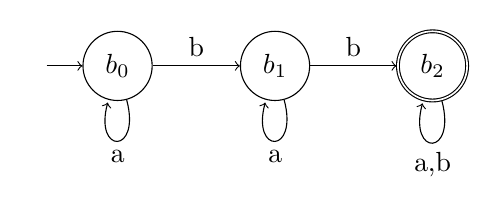
\begin{tikzpicture}[auto, on grid, node distance=2cm, initial text=]
        \node[state, initial]   (b_0)                {$b_0$}; 
        \node[state]            (b_1) [right of=b_0] {$b_1$};
        \node[state, accepting] (b_2) [right of=b_1] {$b_2$}; 
        \path[->] 
          (b_0) edge [loop below] node {a}   ()
                edge []           node {b}   (b_1)
          (b_1) edge [loop below] node {a}   ()
                edge []           node {b}   (b_2)
          (b_2) edge [loop below] node {a,b} ();
        \end{tikzpicture}
      \end{center}
  \end{solution}

\question
  Draw a DFA that accepts all strings over $\{a,b\}$ that have exactly two $a$'s~\cite{sipser96}.
  \begin{solution}
    \begin{center}
      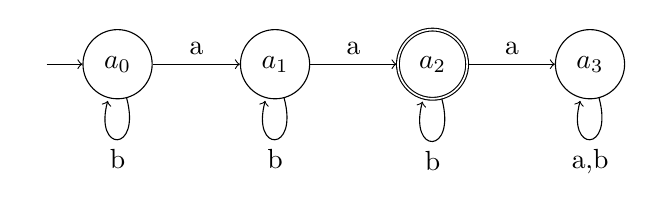
\begin{tikzpicture}[auto, on grid, node distance=2cm, initial text=]
        \node[state, initial]   (a_0)                {$a_0$}; 
        \node[state]            (a_1) [right of=a_0] {$a_1$};
        \node[state, accepting] (a_2) [right of=a_1] {$a_2$}; 
        \node[state]            (a_3) [right of=a_2] {$a_3$};
        \path[->] 
          (a_0) edge [loop below] node {b}   ()
                edge []           node {a}   (a_1)
          (a_1) edge [loop below] node {b}   ()
                edge []           node {a}   (a_2)
          (a_2) edge [loop below] node {b}   ()
                edge []           node {a}   (a_3)
          (a_3) edge [loop below] node {a,b} ();
      \end{tikzpicture}
    \end{center}
  \end{solution}

  \question
  Draw a DFA that accepts all strings over $\{a,b\}$ that have an odd number of $a$'s~\cite{sipser96}.
  \begin{solution}
    \begin{center}
      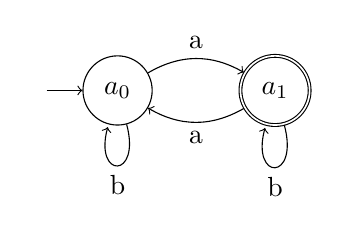
\begin{tikzpicture}[auto, on grid, node distance=2cm, initial text=]
        \node[state, initial]   (a_0)                {$a_0$}; 
        \node[state, accepting] (a_1) [right of=a_0] {$a_1$};
        \path[->]
          (a_0) edge [bend left]  node {a} (a_1)
                edge [loop below] node {b} (a_0)
          (a_1) edge [bend left]  node {a} (a_0)
                edge [loop below] node {b} (a_1);
      \end{tikzpicture}
    \end{center}
\end{solution}

\question
  Draw a DFA that accepts all strings over $\{a,b\}$ that have at least three $a$'s and at least two $b$'s~\cite{sipser96}.
\begin{solution}
  \begin{center}
    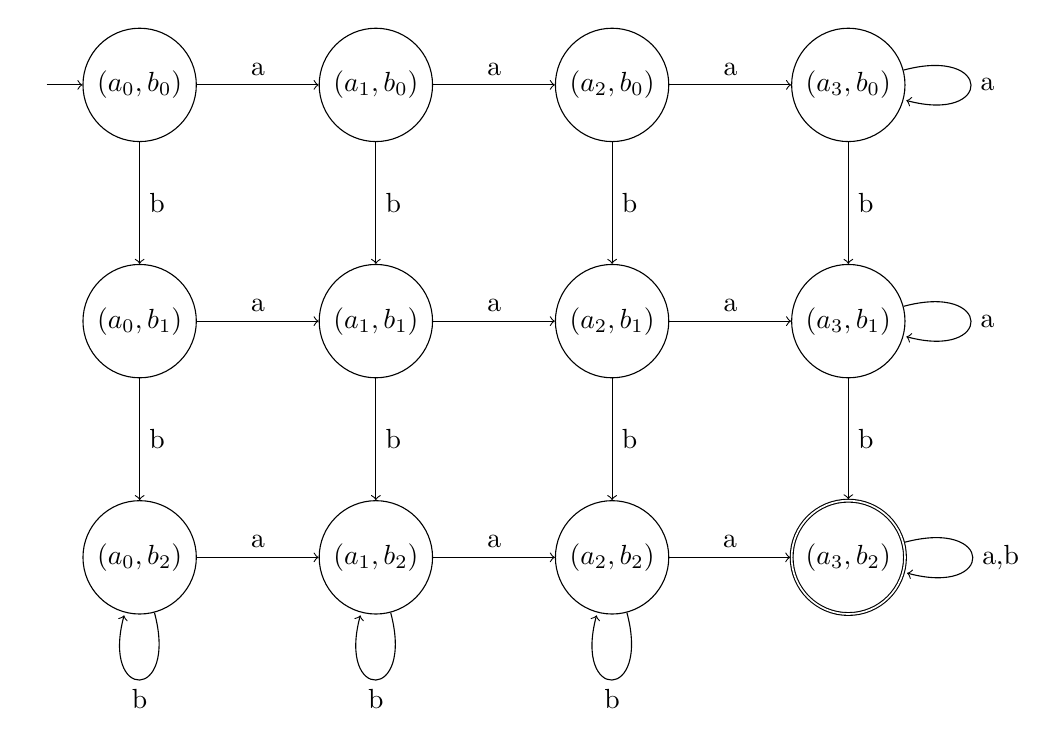
\begin{tikzpicture}[auto, on grid, node distance=3cm, initial text=]
      \node[state, initial]   (a0b0)                 {$(a_0,b_0)$};
      \node[state]            (a1b0) [right of=a0b0] {$(a_1,b_0)$};
      \node[state]            (a2b0) [right of=a1b0] {$(a_2,b_0)$};
      \node[state]            (a3b0) [right of=a2b0] {$(a_3,b_0)$};

      \node[state]            (a0b1) [below of=a0b0] {$(a_0,b_1)$};
      \node[state]            (a1b1) [right of=a0b1] {$(a_1,b_1)$};
      \node[state]            (a2b1) [right of=a1b1] {$(a_2,b_1)$};
      \node[state]            (a3b1) [right of=a2b1] {$(a_3,b_1)$};

      \node[state]            (a0b2) [below of=a0b1] {$(a_0,b_2)$};
      \node[state]            (a1b2) [right of=a0b2] {$(a_1,b_2)$};
      \node[state]            (a2b2) [right of=a1b2] {$(a_2,b_2)$};
      \node[state, accepting] (a3b2) [right of=a2b2] {$(a_3,b_2)$};
      \path[->] 
        (a0b0) edge []           node {a}   (a1b0)
              edge []           node {b}   (a0b1)
        (a0b1) edge []           node {a}   (a1b1)
              edge []           node {b}   (a0b2)
        (a0b2) edge []           node {a}   (a1b2)
              edge [loop below] node {b}   (a0b2)
        (a1b0) edge []           node {a}   (a2b0)
              edge []           node {b}   (a1b1)
        (a1b1) edge []           node {a}   (a2b1)
              edge []           node {b}   (a1b2)
        (a1b2) edge []           node {a}   (a2b2)
              edge [loop below] node {b}   (a1b2)
        (a2b0) edge []           node {a}   (a3b0)
              edge []           node {b}   (a2b1)
        (a2b1) edge []           node {a}   (a3b1)
              edge []           node {b}   (a2b2)
        (a2b2) edge []           node {a}   (a3b2)
              edge [loop below] node {b}   (a2b2)
        (a3b0) edge [loop right] node {a}   (a3b0)
              edge []           node {b}   (a3b1)
        (a3b1) edge [loop right] node {a}   (a3b1)
              edge []           node {b}   (a3b2)
        (a3b2) edge [loop right] node {a,b} (a3b2);
    \end{tikzpicture}
  \end{center}
\end{solution}

\question
  Describe all of the above automata.


\end{questions}

\bibliographystyle{plain}
\bibliography{bibliography}
\end{document}
